\batchmode
\documentclass{beamer}
\usepackage[utf8]{inputenc}
\usepackage[ngerman]{babel}

\usetheme[deutsch]{KIT}

\newcommand{\WProve}{W\tiny{}e\Large{}Prove}

\author{Simon Bischof \and Jan Haag \and Adrian Herrmann \and Lin Jin \and Tobias Schlumberger \and Matthias Schnetz}
\title{\WProve}
\institute{Institut f\"ur Theoretische Informatik}
\TitleImage[scale=0.225]{frontpic.jpg}

\begin{document}
\begin{frame}
\maketitle
\end{frame}

\begin{frame}
\frametitle{Inhalt}
\tableofcontents
\end{frame}

\section{Aufgabenstellung}
\begin{frame}
\frametitle{Aufgabenstellung: Parser und Interpreter}
\begin{center}
\includegraphics[scale=2.5]{images/ParserInterpreter.png}
\end{center}
\end{frame}

\begin{frame}
\frametitle{Aufgabenstellung: Formale Verifikation}
\begin{center}
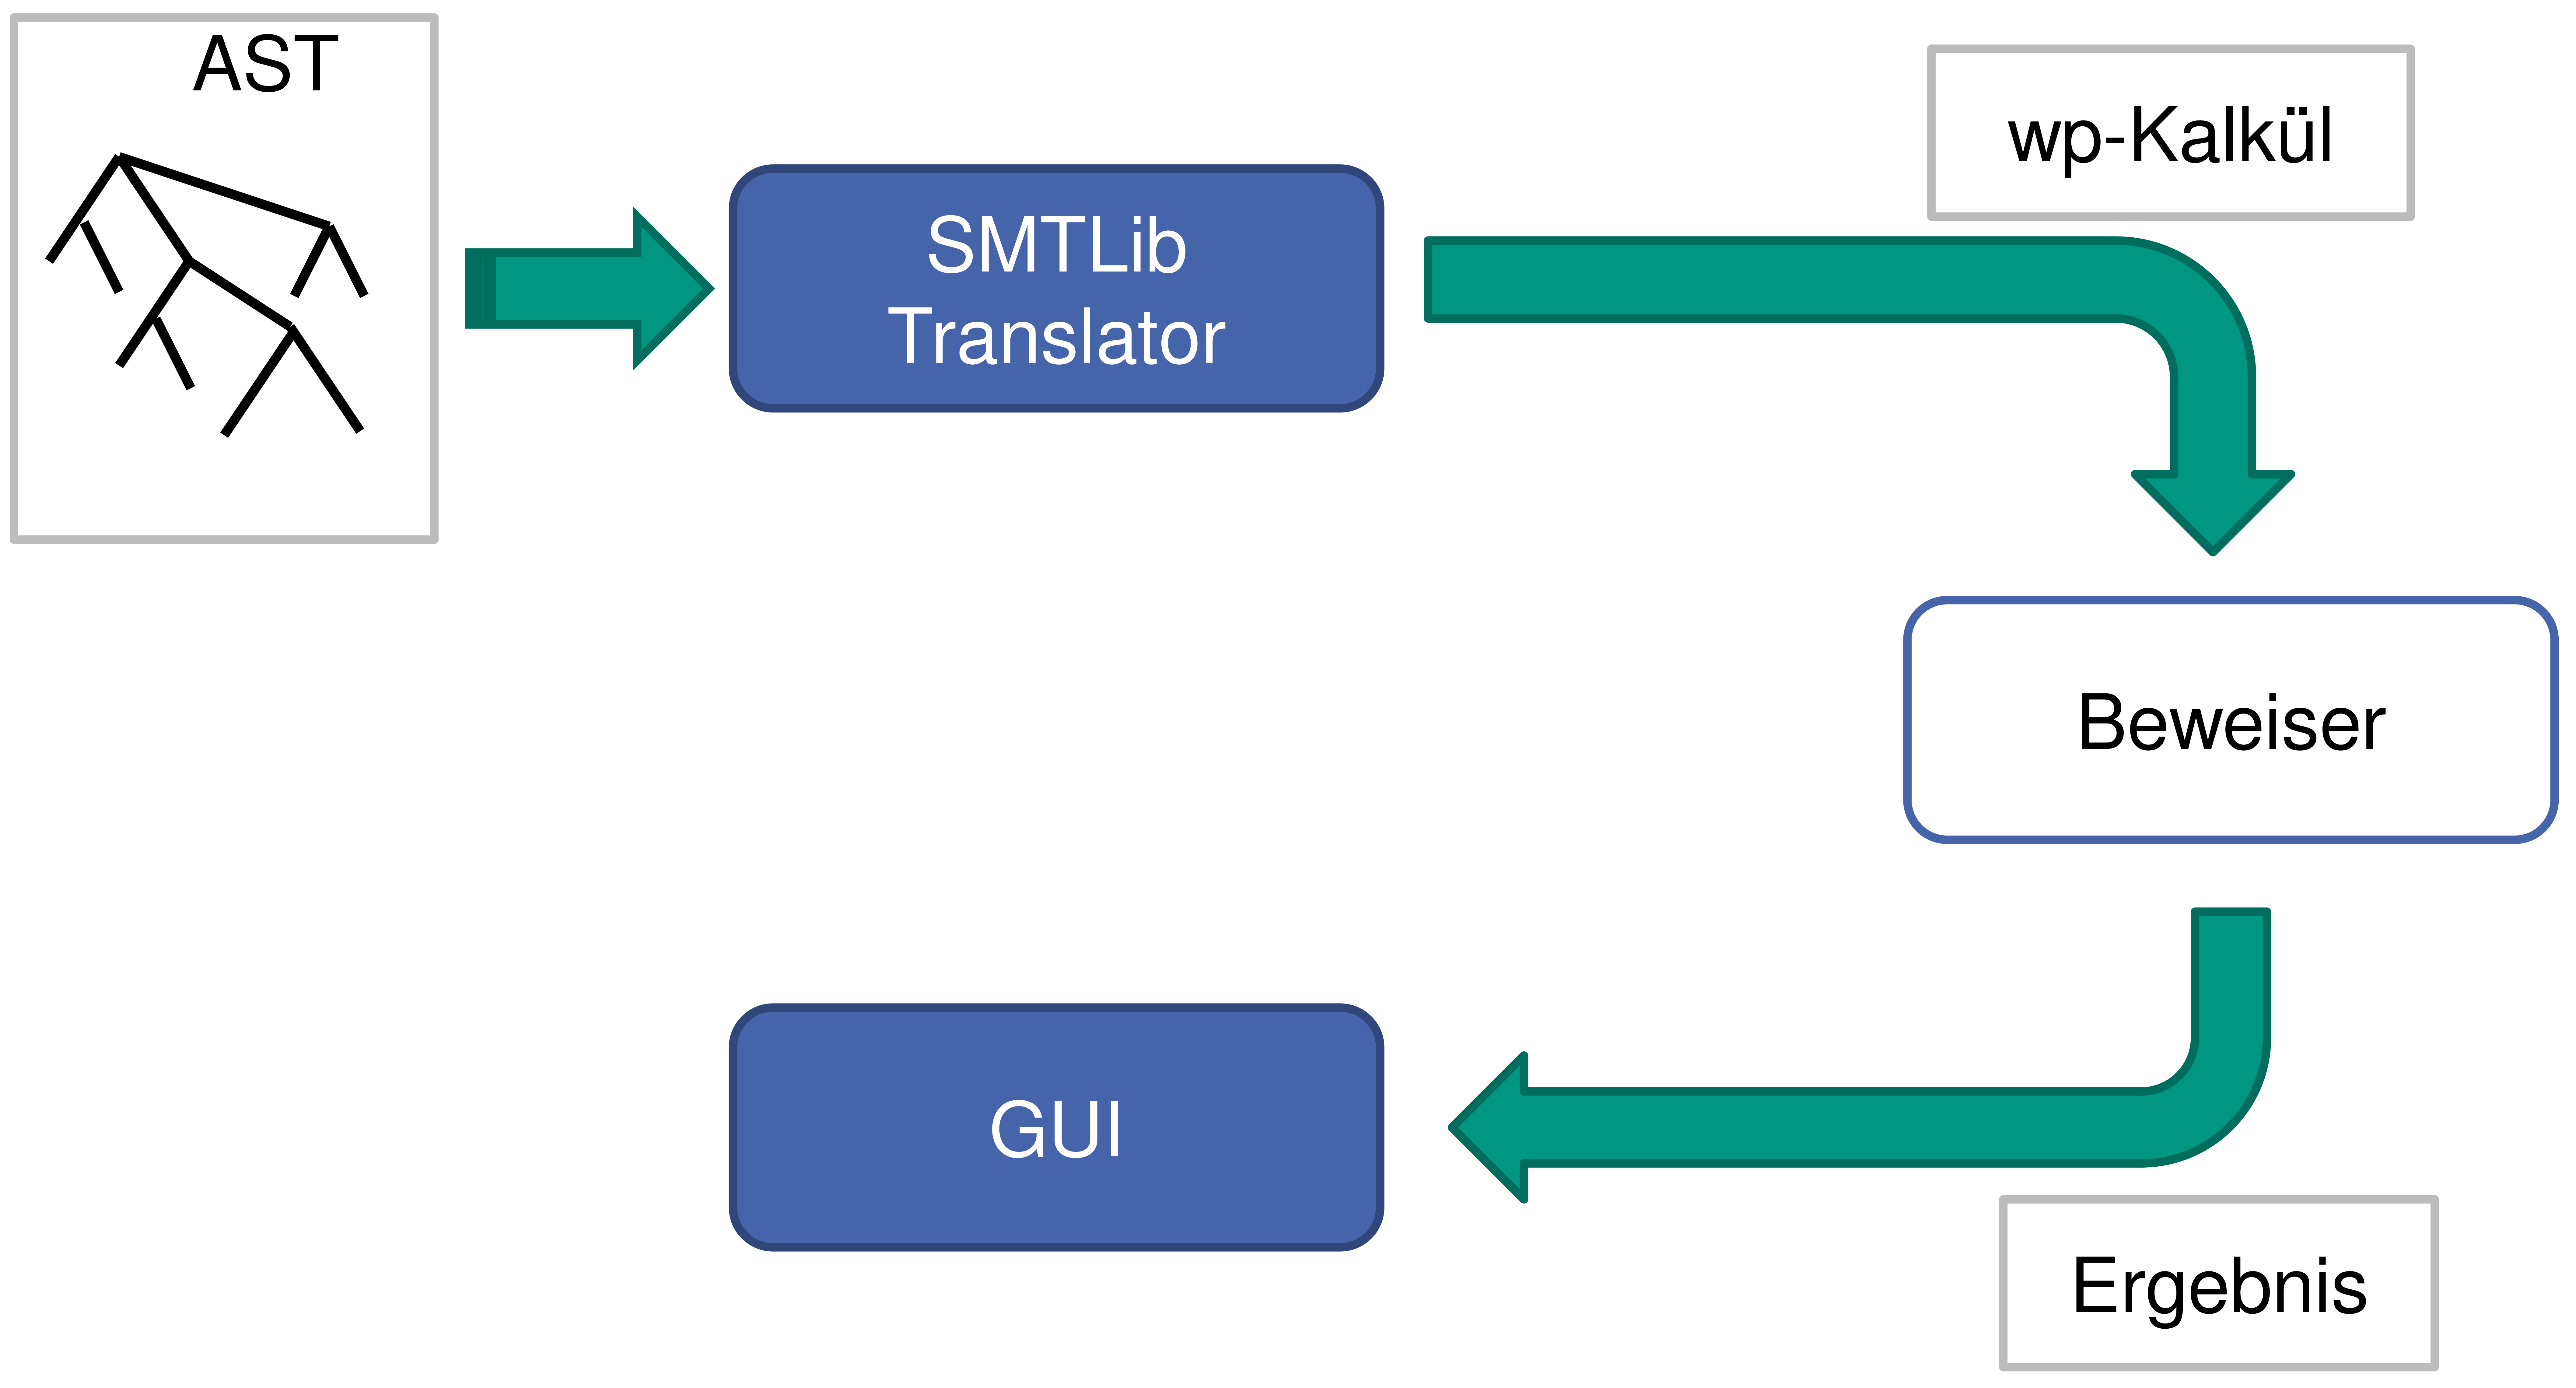
\includegraphics[scale=2.5]{images/SMTLibTranslator.png}
\end{center}
\end{frame}

\begin{frame}
\frametitle{Aufgabenstellung: Formale Verifikation}
Zur Verifikation eines Programmes sind zwei Schritte nötig:
    \begin{enumerate}
    \item<+-> Ziel des Programms kl\"aren
    \begin{itemize}
        \item Was ist der Sinn dieses Programms?
        \item Welches Endergebnis erwarte Ich?
        \item Wie soll dieses Ergebnis erreicht werden?
    \end{itemize}
    \item<+- | visible> Das Programm um beweisbare Annotationen erweitern
    \begin{itemize}
        \item Was gilt für die Variablen?
        \item Wie lauten geeignete Invarianten für Schleifen?
        \end{itemize}
    \end{enumerate}
\end{frame}

\begin{frame}[fragile]
\frametitle{Aufgabenstellung: Formale Verifikation}
\begin{enumerate}
\centering
\begin{overprint}[308pt]
\onslide<1>
\item Ziel des Programms kl\"aren
\begin{itemize}
\item Was ist der Sinn dieses Programms?
\item Welches Endergebnis erwarte Ich?
\item Wie soll dieses Ergebnis erreicht werden?
\end{itemize}
\begin{verbatim}
1. Lorem ipsum dolor sit amet...
\end{verbatim}
\onslide<2>
\item Das Programm um beweisbare Annotationen erweitern
\begin{itemize}
\item Was gilt für die Variablen?
\item Wie lauten geeignete Invarianten für Schleifen?
\end{itemize}
\begin{verbatim}
2. Lorem ipsum dolor sit amet...
\end{verbatim}
\end{overprint}
\end{enumerate}
\end{frame}

\section{Kenndaten}
\begin{frame}
\frametitle{Kenndaten}
\begin{columns}[c]
\column{190pt}
\begin{itemize}
\item 6 Entwickler
\item 17.000 LOC
\begin{itemize}
\item 100 Klassen
\item 15 Pakete
\end{itemize}
\item Lauffähig unter:
\begin{itemize}
\item Windows XP \& Windows 7
\item Linux
\item Mac OS X
\end{itemize}
\item Beweisbare Programme:
\begin{itemize}
\item Summe von 1 bis n
\item Russische Multiplikation
\end{itemize}
\end{itemize}

\column{115pt}
9.500 Zeilen\\
Code\\
\vspace{1\baselineskip}
3.500 Zeilen\\
generierter Code\\
\vspace{1\baselineskip}
3.500 Zeilen\\
Code aus der QS\\
\vspace{1\baselineskip}
800 Zeilen\\
Dokumentation
\end{columns}
\end{frame}

\section{Zukunft von \WProve}
\begin{frame}
\frametitle{Zukunft von \WProve}
\begin{itemize}
\item Einsatzgebiete von formaler Verifikation:
\begin{itemize}
\item Hardware-Bereich: Entwicklung von Prozessoren
\item Software-Bereich: Systeme, deren Zuverlässigkeit wichtig ist
\end{itemize}
\item Es existieren andere Tools mit größerem Funktionsumfang und
Entwicklerteams mit mehr Erfahrung/Mitteln
\begin{itemize}
\item KeY
\item Isabelle/HOL
\end{itemize}
\end{itemize}
\begin{tabular}{p{1mm}p{10.9cm}}
$\Rightarrow$ & Tool ist ein guter Einstieg in den Themenbereich der formalen
Verifikation (v.a. auch für Studenten)\\
$\Rightarrow$ & Lizensierung unter BSD Lizenz
\end{tabular}
\end{frame}

\begin{frame}
\frametitle{Tool Demonstration}
TODO: Bild
\end{frame}

\section{Soll / Haben}
\begin{frame}
\frametitle{Soll / Haben}
\end{frame}


\section{Qualit\"atssicherung}
\begin{frame}
\frametitle{Qualit\"atssicherung}
Werkzeuge:
\begin{itemize}
\item GitHub Bugtracker
\item JUnit
\item GUI-Testplan
\end{itemize}
\vspace{1\baselineskip}
Probleme:
\begin{itemize}
\item Klare Abgrenzung der einzelnen Module zum Teil schwierig
\item Testen von generiertem Code nur teilweise möglich
\end{itemize}
\vspace{1\baselineskip}
\begin{tabular}{p{1mm}p{10.9cm}}
$\Rightarrow$ & 108 gefundene Bugs\\
$\Rightarrow$ & Code Coverage: ca. 90 \%
\end{tabular}
\end{frame}

\begin{frame}
\frametitle{Verteilung der Bugs auf die Module}
TODO: Graphik
\end{frame}

\section{Herausforderungen \& Erfahrungen}
\begin{frame}
\frametitle{Herausforderungen \& Erfahrungen}
\begin{itemize}
\item Herausforderungen
\begin{itemize}
\item Grammatikerstellung für Parser erfordert Behandlung vieler
Spezialfälle
\item Themengebiet der formalen Verifikation sehr abstrakt / komplex
\item In manchen Phasen hoher Zeitdruck
\end{itemize}
\item Erfahrungen
\begin{itemize}
\item Fehler / ungelöste Probleme des Entwurfs wirken sich sehr stark
auf die Implementierung aus
\item Zeitplanung
\item Beteiligung/Engagement schwankt zwischen wenig und viel
\item Qualitätssicherung bringt mehr Fehler zum Vorschein als erwartet
\end{itemize}
\end{itemize}
\end{frame}

\end{document}
